% !TeX encoding=utf8
% !TeX spellcheck = en-US

\chapter{Background}

Combinatorial map is a topological structure describing the rotational graph embedded in the surface. It includes three components: vertices, edges and faces. Each of them is composed of permutations of darts. This section will introduce these concepts and terminology.

\section{Permutations}

Permutation is arranging all members of a set or a sequence with a certain order, and each order called a permutation. For example, the set \{1,2\} have two permutations (1 2) and (2 1).  Each permutation is written as tuple. Three notations can be used to represent this concept, two-line notation, one-line notation and cycle notation.
%
% \begin{equation}
%   J_f(a) := \frac{\partial {f}}{\partial {x}}(a) 
%          := \frac{\partial(f_1,  \ldots, f_m)}{\partial(x_1, \ldots, x_n)}(a)
%          := \left(\frac{\partial f_i(a)}{\partial x_j}\right)_{i=1,\ldots,m;\
%              j=1,\ldots,n}
% \end{equation}

\subsection*{Two-line notation}

As the name implies, this notation uses two rows two indicate the permutations. The first row is the list of elements in set , for instance, the first row of set \{1,2,3\} would be (1 2 3). Meanwhile, the second line is its permutations, hence the second line for the example is (3 2 1). The permutation (3 2 1) can be written as \(p=\bigl( 
  \begin{smallmatrix}
    1 & 2 & 3 \\
    3 & 2 & 1
   \end{smallmatrix}
   \bigr)\). From the example we could see that that this notation shows permutations quite clear and intuitive. The permutation which is represented by this notation can be drew as the \cref{fig:figures:twolineperm}. In the \cref{fig:figures:twolineperm}, it is obvious that the permutation is a mapping for set  to itself, so that it can be defined as a function \(p\). Take the example (3 2 1) again, the second line of it can be written as \((p(1),p(2),p(3))\) where \(p(1)=3\), \(p(2)=2\) and \(p(3)=1\), as well as, the whole formula for the example can be rewritten as \(p=\bigl( 
    \begin{smallmatrix}
      1 & 2 & 3 \\
      p(1) & p(2) & p(3)
     \end{smallmatrix}
     \bigr)\). 

    \begin{figure}[htb]
      \centering
      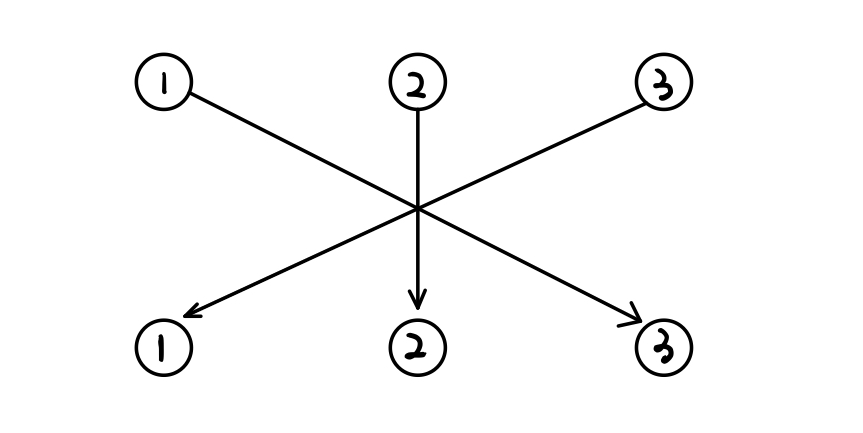
\includegraphics[width=0.5\textwidth]{../../image/twolineperm.png}
      \caption{Two-line notation for permutation \(p=(3\,2\,1)\),in which \(p(1)=3\), \(p(2)=2\) and \(p(3)=1\).}
      \label{fig:figures:twolineperm}
    \end{figure}

\subsection*{One-line notation}

Generally, the first row in two-line notation is a list of set with ascending order, thus, the first line can be omitted and only retaining the second row, which called one-line notation. According to the second line in two-line notation, this notation is \((p(1)\,p(2)\,P(3)\,...)\). This format has occurred more than once in the example mentioned above as (3 2 1).

\subsection*{Cycle notation}

The permutation can be divided into disjoint cycles with the help of applying the permutation to members in set \(S\) again and again. The formula is described as \((x1\,p(x1)\,p(p(x1))\,...)\) which means that the arbitrary element \(x1\) in \(S\) is chose as the start of a cycle and the result \(p(x1)\) would be the next member in the cycle. The third one is applying \(p\) to \(p(x1)\) again. Repeating steps until return the first element . We still using the permutation \(p=(3\,2\,1)\) as example, it has two cycles (1 3) and (2). In the former cycle, the element 1 is applied to the  and we get \(p(1)=3\), after that, the consequence of applying \(p\) to 3 is 1 again, thus, (1,3) is the final result. The same can be proved that (2) is the second cycle. The equation between one-line notation and cycle notation is \(p=(3\,2\,1)=(1\,3)(2)\). The \cref{fig:figures:cycleperm} shows the cycle notation. This notation make a transparent structure of permutation.

\begin{figure}[htb]
  \centering
  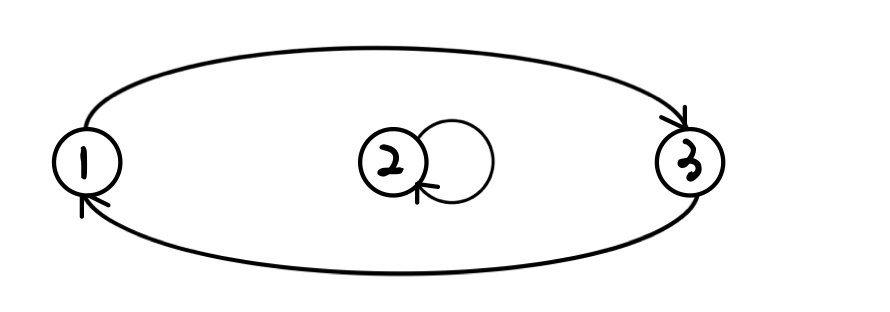
\includegraphics[width=0.5\textwidth]{../../image/cycleperm.png}
  \caption{Cycle notation for permutation \(p=(3\,2\,1)=(1\,3)(2)\).}
  \label{fig:figures:cycleperm}
\end{figure}

\section{Combinatorial maps}

Combinatorial map using oriented subdivided objects to represent the graph embedded in the surface. At the beginning, the concept appeared for the planar graphs of polyhedral surfaces by J. Edmonds \cite{edmonds1960combinatorial} and named as “Constellations” \cite{jacques1969constellations} and “rotation” \cite{ringel2012map} by  A. Jacques and Gerhard Ringel, respectively. The concept is extended from 2-dimensional objects to higher-dimensional objects and called “combinatorial maps” formally.

Sometimes, the computer needs to use data structure to indicate the subdivision of an object and the relation between each of them. The embedded graphs into the surfaces which are assumed to be connected, oriented and compact\cite{nlab:map}, have three typical subdivision, vertices, edges and faces. Each of them are represented by a set of permutations of darts.  

\subsection{Darts}
The combinatorial map is an edges-central model. All edges are divided into two parallel lines with arrow to indicate inverse directions, which called darts or half-edges. The main difference between darts and half-edges is the later one only segment the edges directly without using arrow and parallel lines. The \cref{fig:figures:cycleperm} explain this concept and two formats for it.

\begin{figure}[htb]
  \centering
  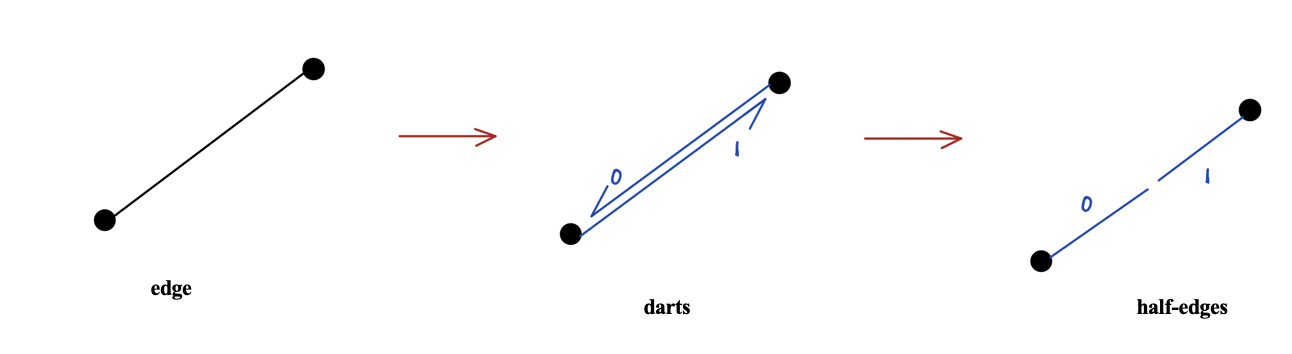
\includegraphics[width=0.8\textwidth]{../../image/darts.png}
  \caption{Two formats of the darts (half-edges) structure.}
  \label{fig:figures:darts}
\end{figure}

\subsection{Edges}
It is obvious that an edges can be represented by a pair of darts. Assume that there is a set of darts \{0,1\} and from the picture we found that dart “0” toward to “1”, on the contrary, dart “1” return to “0”. This means the edges have the orientation for anti-clockwise, it shows a permutation of darts can be used to indicate an edges, as well. One-line notation for the example is (1 0), and convert it to the cycle notation as (0 1). The permutation of edges is denoted as \(\alpha\).

\subsection{Vertices}
A vertex consists of incidence darts surrounding it, which also follows the anti-clockwise and using \(\sigma\) denote this component. As the example in the \cref{fig:figures:vertex}, the vertex can be indicated as (0 1 2) under cycle notation.

\begin{figure}[htb]
  \centering
  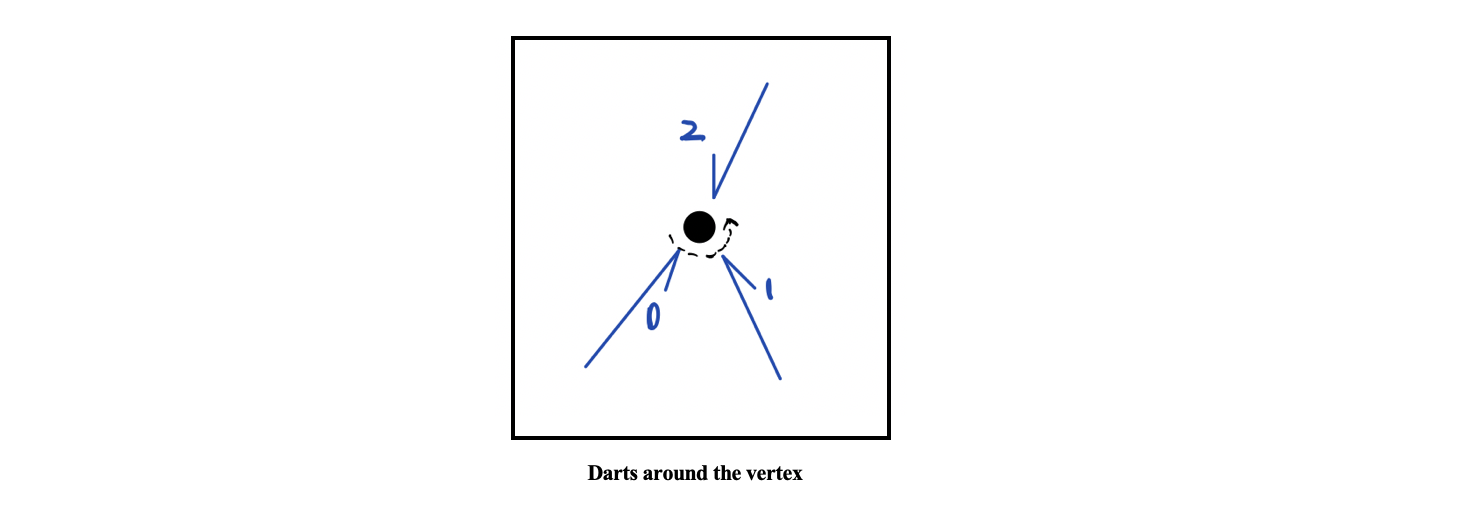
\includegraphics[width=0.8\textwidth]{../../image/vertex.png}
  \caption{The darts surrounding a vertex.}
  \label{fig:figures:vertex}
\end{figure}

\subsection{Faces}
There are two types of faces, the internal faces and the external faces. Both of them are the area surrounded by a series of darts, in other words, both of them have directions. The orientation of the internal faces is clockwise, while for the external ones is anti-clockwise. The signal \(\phi\) is used to indicate the permutation of faces. There are two kinds of faces in the \cref{fig:figures:faces}. (a) has normal faces whose internal face is (0 4 2) and external face is (1 3 5). (b) is a loop which also has the internal face (0) and external one (1). All of the permutations that are mentioned in this section use cycle notation.

\begin{figure}[htb]
  \centering
  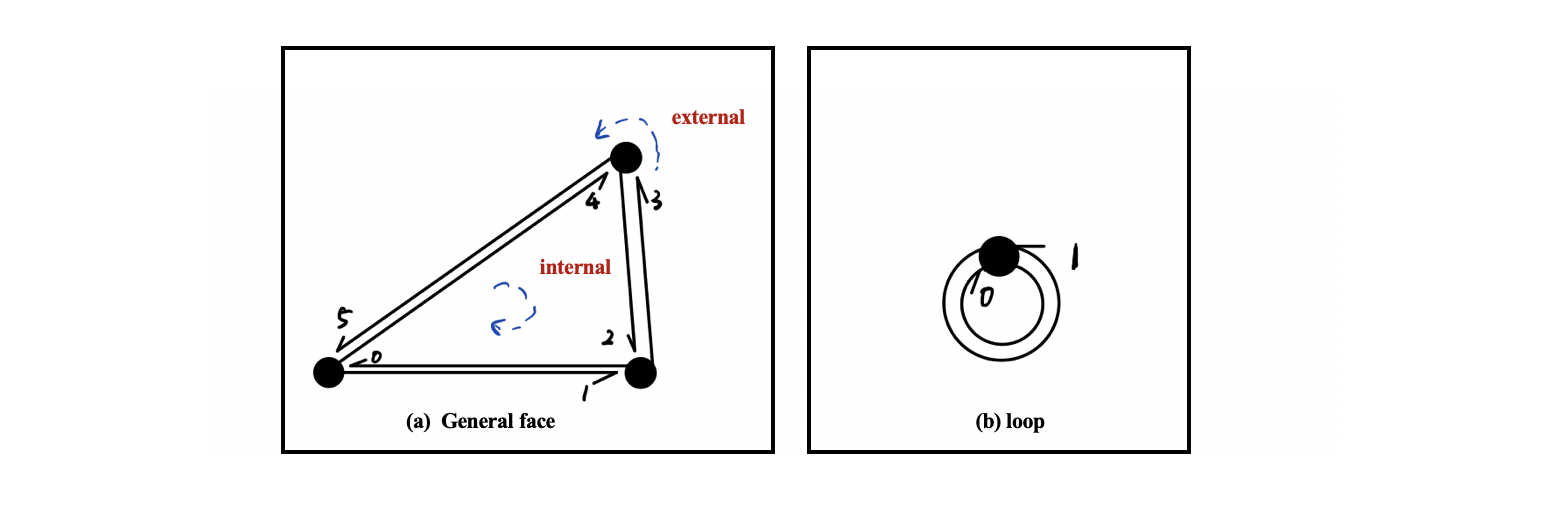
\includegraphics[width=0.8\textwidth]{../../image/face.png}
  \caption{Faces}
  \label{fig:figures:faces}
\end{figure}

\subsection{Planar maps}
Primely, with the requirement of expressing the submission of planar graphs, a compactness topological model  combinatorial map had been utilized. All of  the three component vertices, edges and faces can be tidy and structural represented under an infinite set of darts. \cref{fig:figures:map} draws a typical planar map with format of combinatorial map \(M=(D,\sigma,\alpha)\) in which \(D\) is the infinite set of darts. The length of \(D\) is 14. 

\begin{figure}[htb]
  \centering
  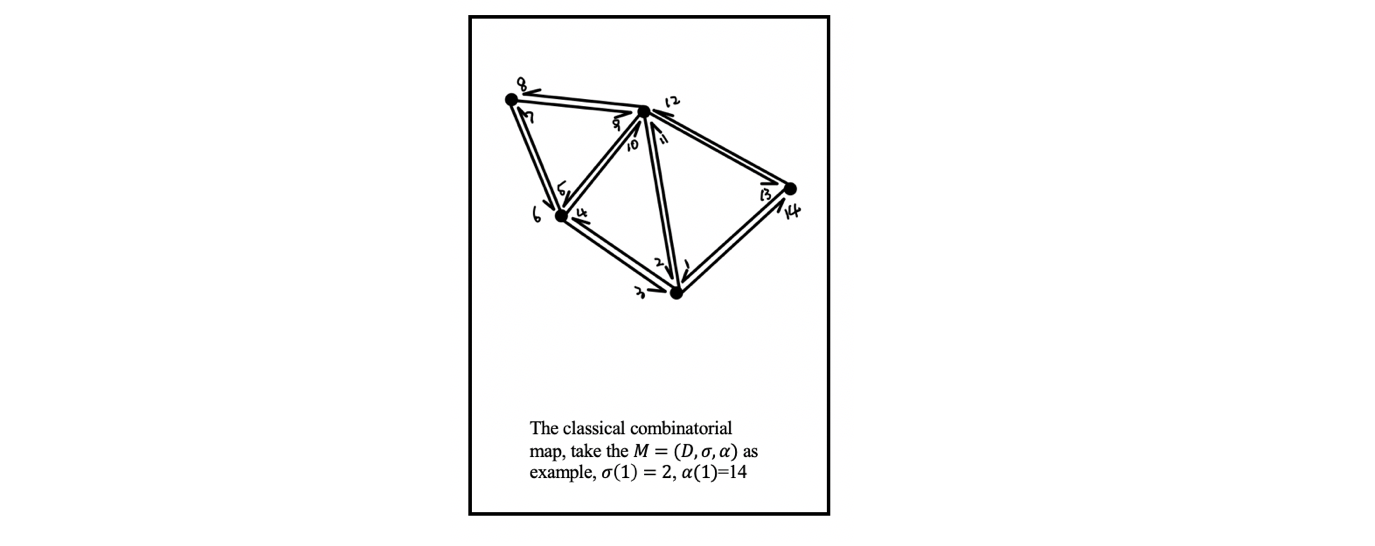
\includegraphics[width=0.8\textwidth]{../../image/map.png}
  \caption{A classical  combinatorial map for a planar map.}
  \label{fig:figures:map}
\end{figure}

Firstly, the permutation of darts for vertices is \(\sigma=(1\,2\,3)(4\,5\,6)(7\,8)(9\,10\,11\,12)(13\,14)=(2\,3\,1\,5\,6\,4\,8\,7\,10\,11\,12\,9\,14\,13)\) , hence, \(\sigma(1)=2\), \(\sigma(2)=3\),etc. The edges permutation is \(\alpha=(1\,14)(2\,11)(3\,4)(5\,10)(6\,7)(8
\,9)(12\,13)=(14\,11\,4\,3\,10\,7\,6\,9\,8\,5\,2\,13\,12\,1)\) where \(\alpha(1)=14\), \(\alpha(2)=11\),etc. Actually, we have a triple of permutations \(<\sigma,\alpha,\phi>\) on \(D\), and the composition of them is identity, which means \(\phi\alpha\sigma=id\). Accordingly, the permutation of faces is calculated as \(\phi=\sigma o \alpha=(1\,11\,13)(2\,4\,10)(3\,14\,12\,8\,6)(5\,7\,9)\).

The orientation of each component is a quite strict constrain to define a combinatorial maps. The definition for discussing whether two maps are conjugation equivalent is only if they are isomorphic by a homeomorphism of the underlying surfaces. That is to say, judging the equivalent of two maps relies on if corresponding parts of those are obey the same rotation, rather than they have the same number of elements for the each component. In the \cref{fig:figures:equivalent}, although the three combinatorial maps have the same number of vertices, edges and faces, the first two a equivalent, and the last one is not the same with them.

\begin{figure}[htb]
  \centering
  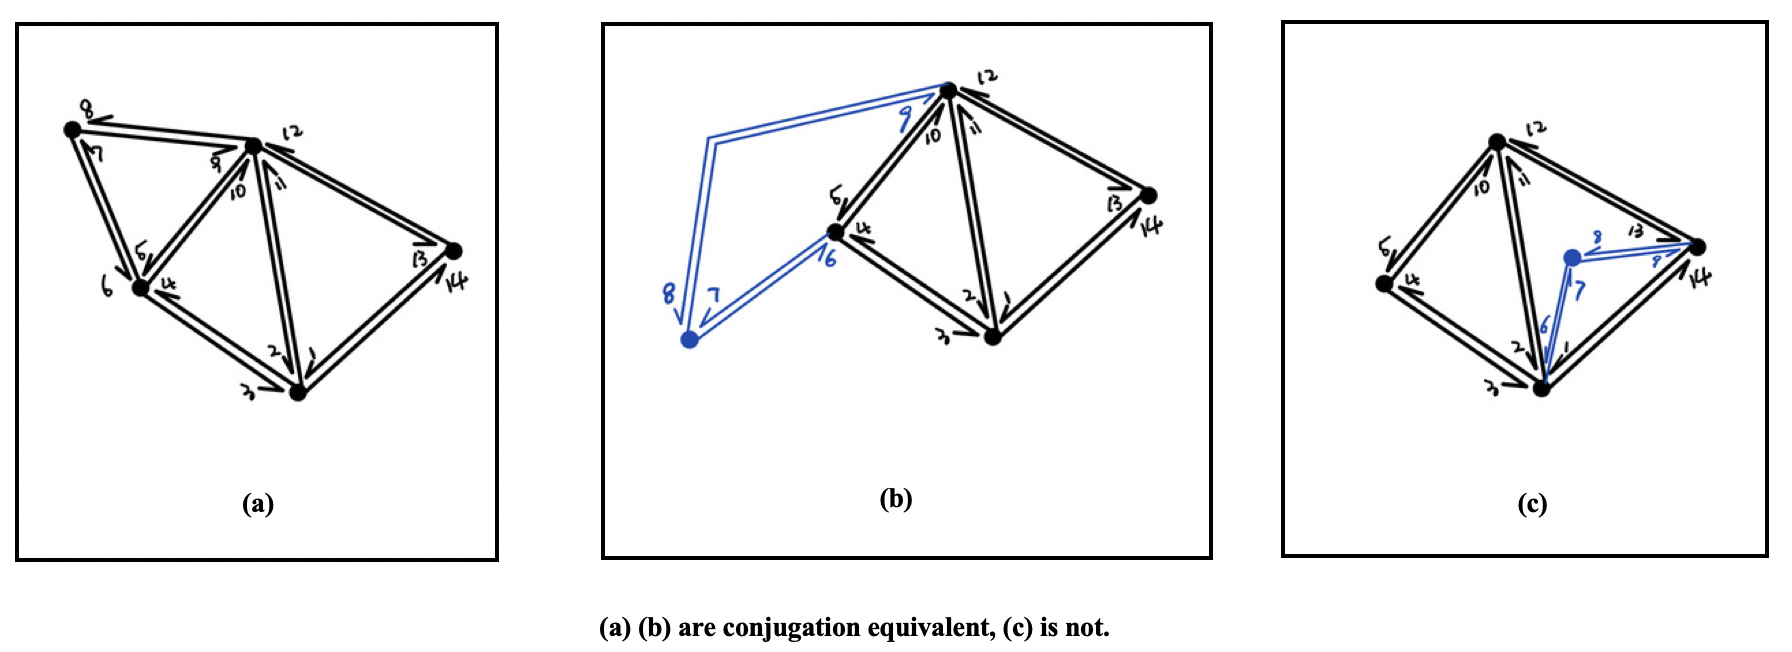
\includegraphics[width=0.8\textwidth]{../../image/equivalent.png}
  \caption{The equivalent of the combinatorial maps.}
  \label{fig:figures:equivalent}
\end{figure}

\subsection{Genus}
An orientable surface might have “holes” , and the number of “holes” it has called genus. For example, sphere as (a) in \cref{fig:figures:orsurfaces} has 0 genus and torus as (b) which looks like a donut has 1genus. The genus \(g\) of a surface which the graph embedded in can be computed by the Euler-Poincaré formula \cite{richeson2008euler}:\(V-E+F=2-2g\). The \(V\), \(E\) and \(F\) are the number of vertices, edges and faces in the embedded graph, respectively. Substituting , \(V\), \(E\) and \(F\) in the equation for features of combinatorial map as \(c(\sigma)-c(\alpha)+c(\phi)=2-2g\). The \(c\) is the function to calculate the count of the cycles for each component.

\begin{figure}[htb]
  \centering
  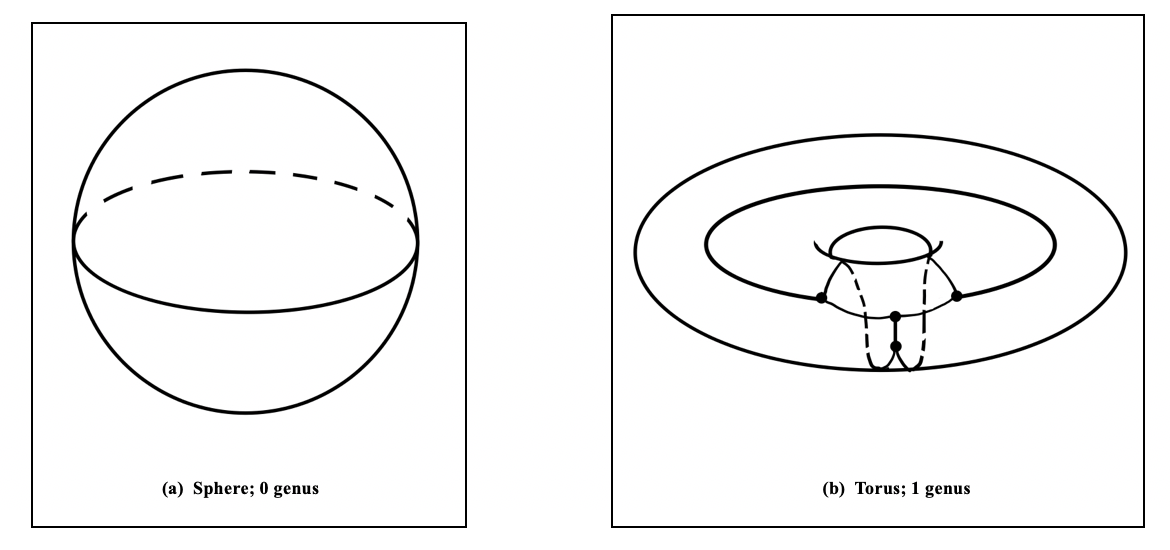
\includegraphics[width=0.8\textwidth]{../../image/oritation surface.png}
  \caption{Two oriented surfaces.}
  \label{fig:figures:orsurfaces}
\end{figure}

\subsection{Generalised maps}
Planar graph is the graph embedded in a plane surface which has 0 genus. It is a crossing free model and the combinatorial map for it is also named 2-dimensional map. Gradually, the combinatorial map is discovered not only to represent the planar maps, but to indict more complicate objects with higher-dimension, even the non-orientation surfaces. The triple of permutations \(<\sigma,\alpha,\phi>\) on set \(D\) is still used to describe the subdivision of the objects.  Take the torus as the example, in \cref{fig:figures:hdmap}, the embedded graph on this oriented surface drew like (b), and the labels are half-edges. The permutation for edges is  \(\alpha=(1\,8)(2\,11)(3\,4)(5\,12)(6\,7)(9\,10)\) and for vertices is \(\sigma=(1\,2\,3)(4\,5\,6)(7\,8\,9)(10\,11\,12)\). (c) is the isomorphic map for the graph.

\begin{figure}[htb]
  \centering
  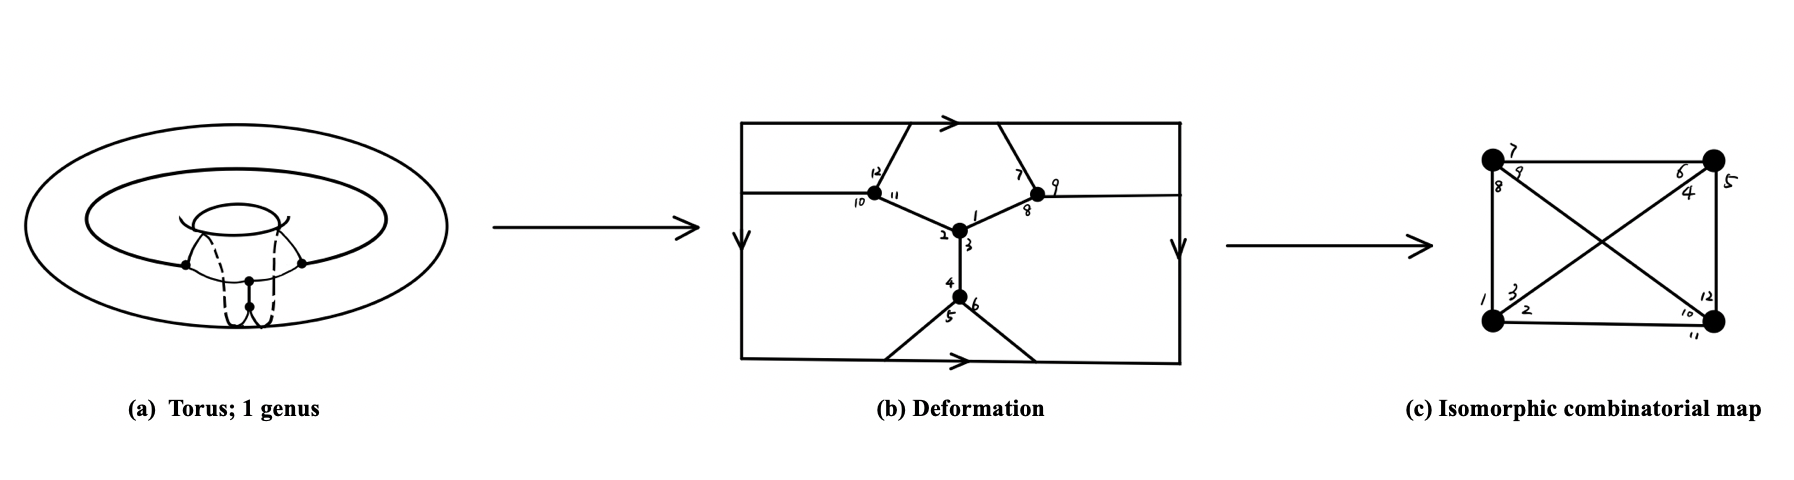
\includegraphics[width=0.8\textwidth]{../../image/hdmap.png}
  \caption{Combinatorial map for torus.}
  \label{fig:figures:hdmap}
\end{figure}

As far, the combinatorial maps can be used to indict a lot of objects with tidy and direct structure. It also involve into the field of graph drawing and hierarchical image partitioning \cite{haxhimusa2005hierarchical}. Some graph algorithm library like Pigale \cite{de2002pigale} use the structure as the basic data structure.